\section{Interpretability (RQ4)}
SHAP values describe how the fitted model uses its inputs. They are associational, not causal, and agreement with clinical knowledge is necessary but not sufficient evidence of validity (Section~II-D). We therefore report the explanations together with their stability, and we propose review by cardiologists as the appropriate next validation step.

\subsection{Global Feature Ranking}
Fig.~\ref{fig:shapglobal} (v4) shows the global TreeSHAP ranking of the XGBoost member on the seed-42 hold-out. Thallium scan result (\texttt{thal}), number of fluoroscopy-visible vessels (\texttt{ca}), chest-pain type (\texttt{cp}) and ST depression (\texttt{oldpeak}) dominate. This is consistent with clinical knowledge: a perfusion defect on thallium scintigraphy indicates ischaemia or scar, and vessels visualised on fluoroscopy reflect the coronary anatomy that the angiographic label describes. It also needs to be read with care. \texttt{ca} (vessels coloured by fluoroscopy) and \texttt{thal} (thallium stress scintigraphy) are results of advanced diagnostic tests carried out during the same diagnostic work-up that produced the angiographic label. A model that relies on them is a \emph{post-test} classifier, not a screening tool for patients who have not yet had these tests.

\begin{figure}[!t]
\centering
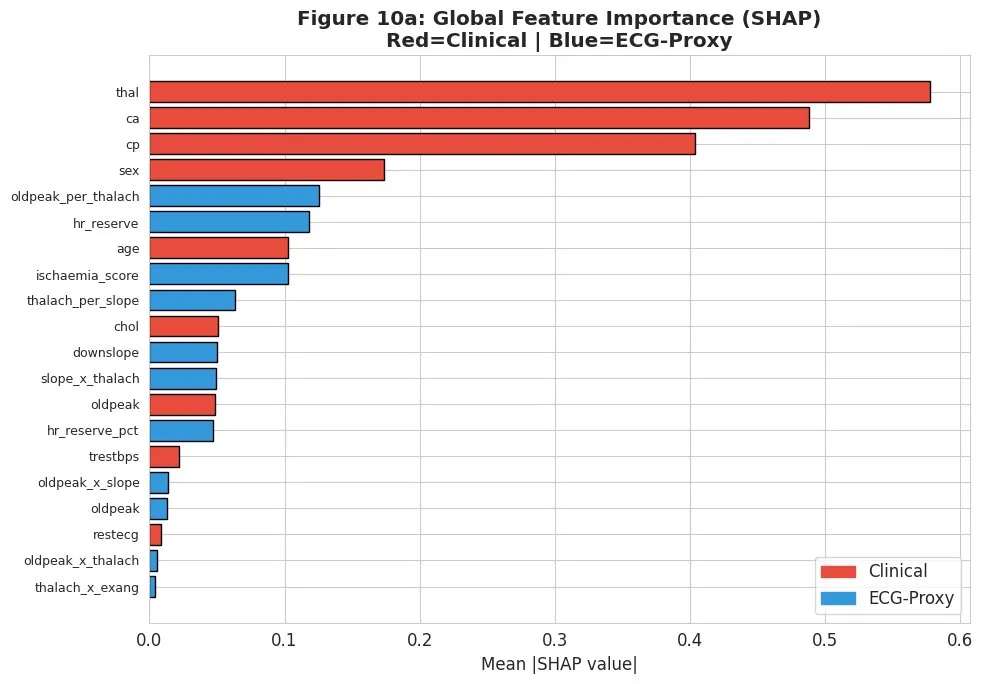
\includegraphics[width=0.92\linewidth]{fig4_shap_global.png}
\caption{Global SHAP importance of the XGBoost member on the v4 hold-out (red = clinical, blue = ECG-proxy).}
\label{fig:shapglobal}
\end{figure}

\subsection{Stability of the Ranking}
Repeating TreeSHAP in each of the 50 CV folds (Table~\ref{tab:e8}, Table~\ref{tab:shaptop}, Fig.~\ref{fig:a7}) shows that the \emph{top} of the ranking is stable while the tail is not. The fold-to-fold Spearman correlation of all 36 feature ranks is \shapRhoFold{}, and the top-5 sets overlap with a mean Jaccard index of \shapJac{}. Across ten training seeds on the full data the ranking correlation is \shapRhoSeed{}. Agreement with permutation importance on the same test folds is lower (Spearman \shapRhoPI{}). This is expected for correlated features: SHAP shares credit among correlated features, whereas permuting one of them leaves the information available through the others.

Under repeated CV, \texttt{cp}, \texttt{ca} and \texttt{thal} are in the top five in every fold (Table~\ref{tab:shaptop}). The ECG-proxy block nevertheless receives about a quarter of the total $|$SHAP$|$ mass, although removing it does not change AUC (Section~VI-A). The clearest case is \texttt{ischaemia\_score}, a product of \texttt{oldpeak}, \texttt{slope} and \texttt{exang}. It ranks fourth by mean $|$SHAP$|$ but its permutation importance is close to zero, and the raw \texttt{oldpeak} column itself falls far down the ranking because its derived terms absorb the credit. The duplicated columns show the same effect: \texttt{oldpeak}, \texttt{thalach}, \texttt{slope}, \texttt{exang} and \texttt{restecg} each appear twice in D3 and their attribution is split between identical copies (on average \dupShareMean{} goes to the proxy copy). The apparent importance of ``ECG-proxy'' features in Fig.~\ref{fig:shapglobal} is therefore \emph{redistributed} importance of the clinical exercise-test variables, not new information. SHAP rankings on engineered features should not be read as evidence that the engineering adds predictive value.

\begin{table}[!t]
\centering
\scriptsize
\caption{Stability of TreeSHAP attributions (XGBoost member) across 50 CV folds and 10 seeds.}
\label{tab:e8}
\setlength{\tabcolsep}{3pt}
\begin{adjustbox}{max width=\linewidth}
\begin{tabular}{lc}
\toprule
Stability measure & Mean (2.5--97.5\%) \\
\midrule
Spearman $\rho$ of SHAP rankings, fold vs fold (all 36 features) & 0.898 (2.5--97.5\%: 0.808--0.953) \\
Jaccard overlap of top-5 SHAP features, fold vs fold & 0.742 (2.5--97.5\%: 0.429--1.000) \\
Spearman $\rho$ of SHAP rankings, seed vs seed (full data) & 0.949 (2.5--97.5\%: 0.925--0.976) \\
Spearman $\rho$, SHAP vs permutation importance (same fold) & 0.270 (2.5--97.5\%: -0.273--0.761) \\
\bottomrule
\end{tabular}
\end{adjustbox}
\end{table}

\begin{table}[!t]
\centering
\scriptsize
\caption{Top-10 features by mean $|$SHAP$|$ over 50 folds, with rank stability and permutation importance (AUC drop).}
\label{tab:shaptop}
\setlength{\tabcolsep}{3pt}
\begin{adjustbox}{max width=\linewidth}
\begin{tabular}{llcccc}
\toprule
Feature & Block & Mean $|$SHAP$|$ & Median rank (IQR) & Top-5 & Perm.\ imp. \\
\midrule
cp & clinical & 0.515 & 2 (1--2) & 100\% & 0.0344 \\
ca & clinical & 0.498 & 2 (1--3) & 100\% & 0.0524 \\
thal & clinical & 0.453 & 3 (2--3) & 100\% & 0.0354 \\
ischaemia\_score & ECG-proxy & 0.162 & 4 (4--5) & 92\% & 0.0037 \\
sex & clinical & 0.119 & 6 (5--7) & 50\% & 0.0101 \\
age & clinical & 0.098 & 7 (5--8) & 28\% & 0.0043 \\
oldpeak\_per\_thalach & ECG-proxy & 0.093 & 7 (6--8) & 22\% & 0.0043 \\
hr\_reserve & ECG-proxy & 0.065 & 9 (8--11) & 2\% & 0.0002 \\
thalach\_per\_slope & ECG-proxy & 0.054 & 11 (9--14) & 2\% & -0.0018 \\
hr\_reserve\_pct & ECG-proxy & 0.052 & 11 (9--13) & 0\% & -0.0007 \\
\bottomrule
\end{tabular}
\end{adjustbox}
\end{table}


\begin{figure}[!t]
\centering
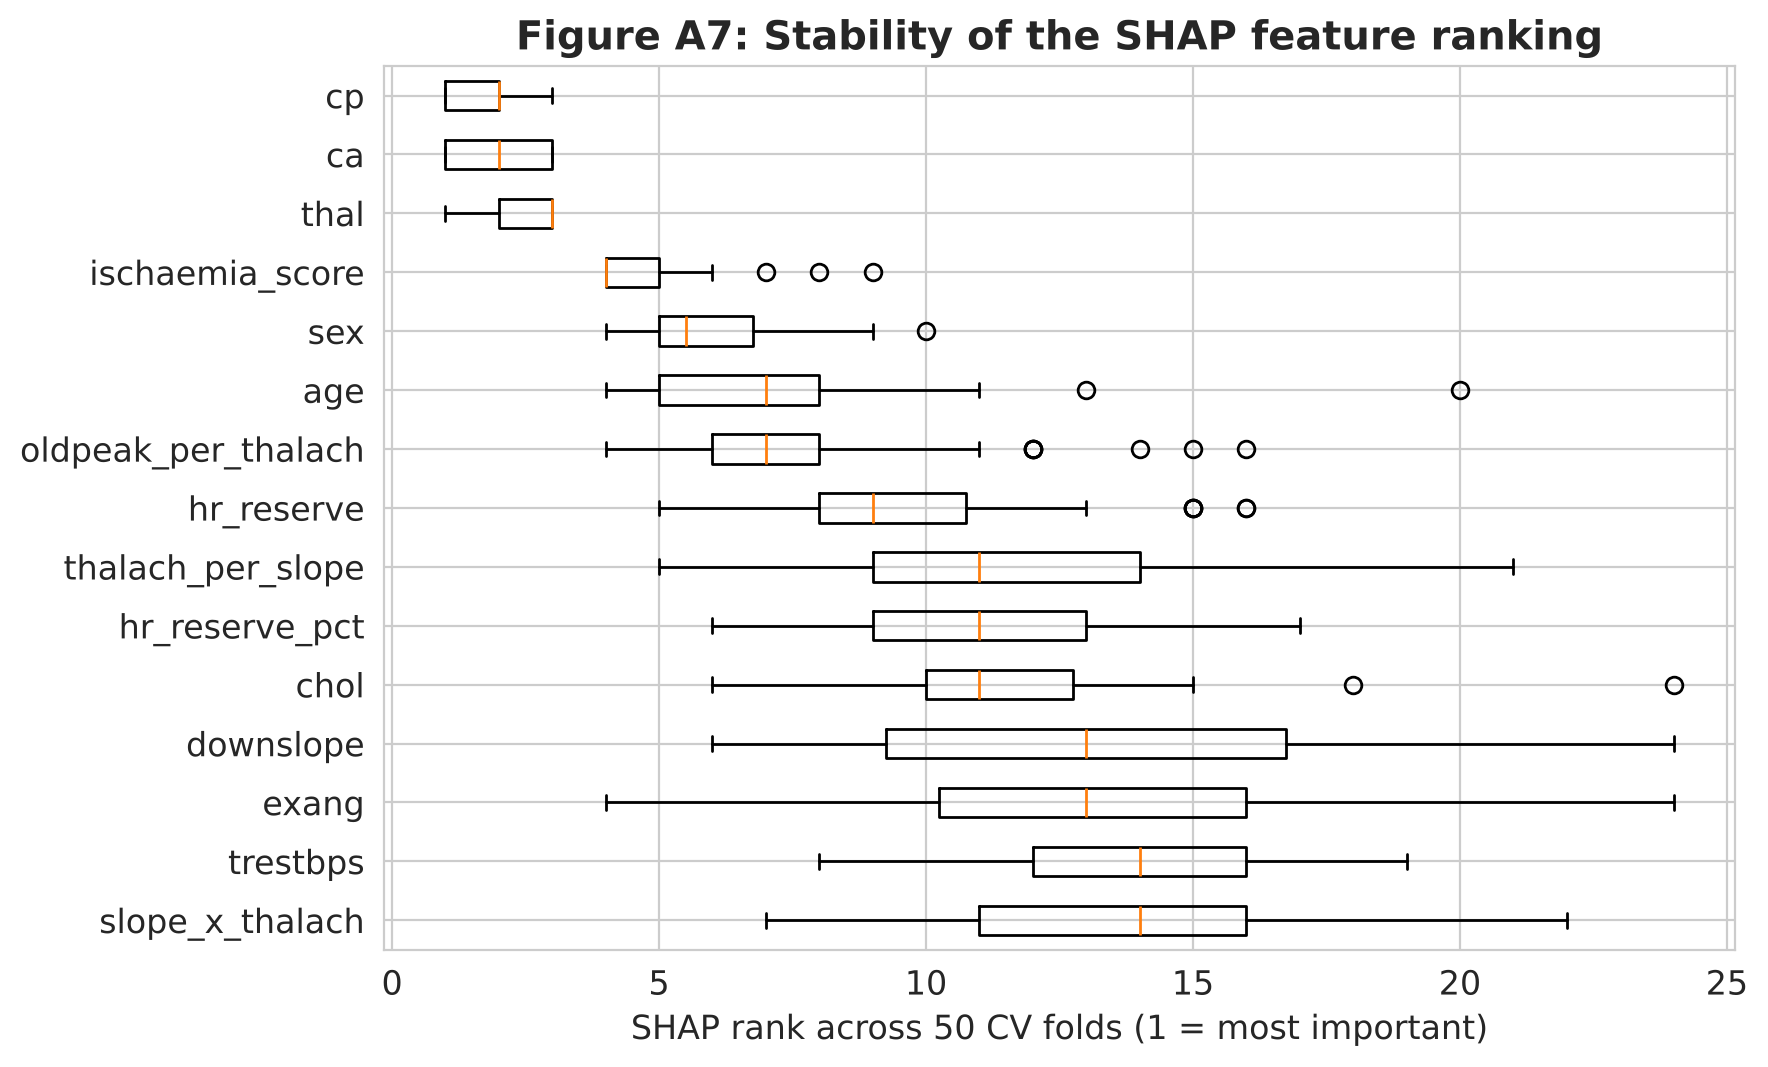
\includegraphics[width=\linewidth]{figA7_shap_rank_stability.png}
\caption{Distribution of each feature's SHAP rank across 50 CV folds.}
\label{fig:a7}
\end{figure}

\subsection{Dependence and Local Explanations}
Dependence plots (Fig.~\ref{fig:a8}) show directions consistent with clinical expectations. Risk rises with ST depression (\texttt{oldpeak}) and falls with higher maximal heart rate. It is higher for both fixed (6) and reversible (7) thallium defects than for a normal scan (3), and higher for asymptomatic chest pain (cp $=4$) than for the three symptomatic types. For \texttt{ca} the effect is essentially a step between 0 and $\geq$1 vessels, with little further increase for 2 or 3 vessels. The higher risk with asymptomatic chest pain reflects the referral population of this cohort, in which 73\% of patients without chest pain had CAD. It should not be read as a general clinical rule. Fig.~\ref{fig:a9} shows local explanations for one true-positive, false-negative, false-positive and true-negative patient. The false negative is a CAD patient whose chest-pain type, vessel count and thallium result all look benign (all three push the prediction towards ``healthy''); this failure mode cannot be fixed by ECG-proxy features derived from the same exercise test. The v4 interaction heatmap (Fig.~\ref{fig:heatmap}) is retained. Its clusters (oldpeak with its derived terms; thalach with slope products) arise largely because these features are functions of each other.

\begin{figure*}[!t]
\centering
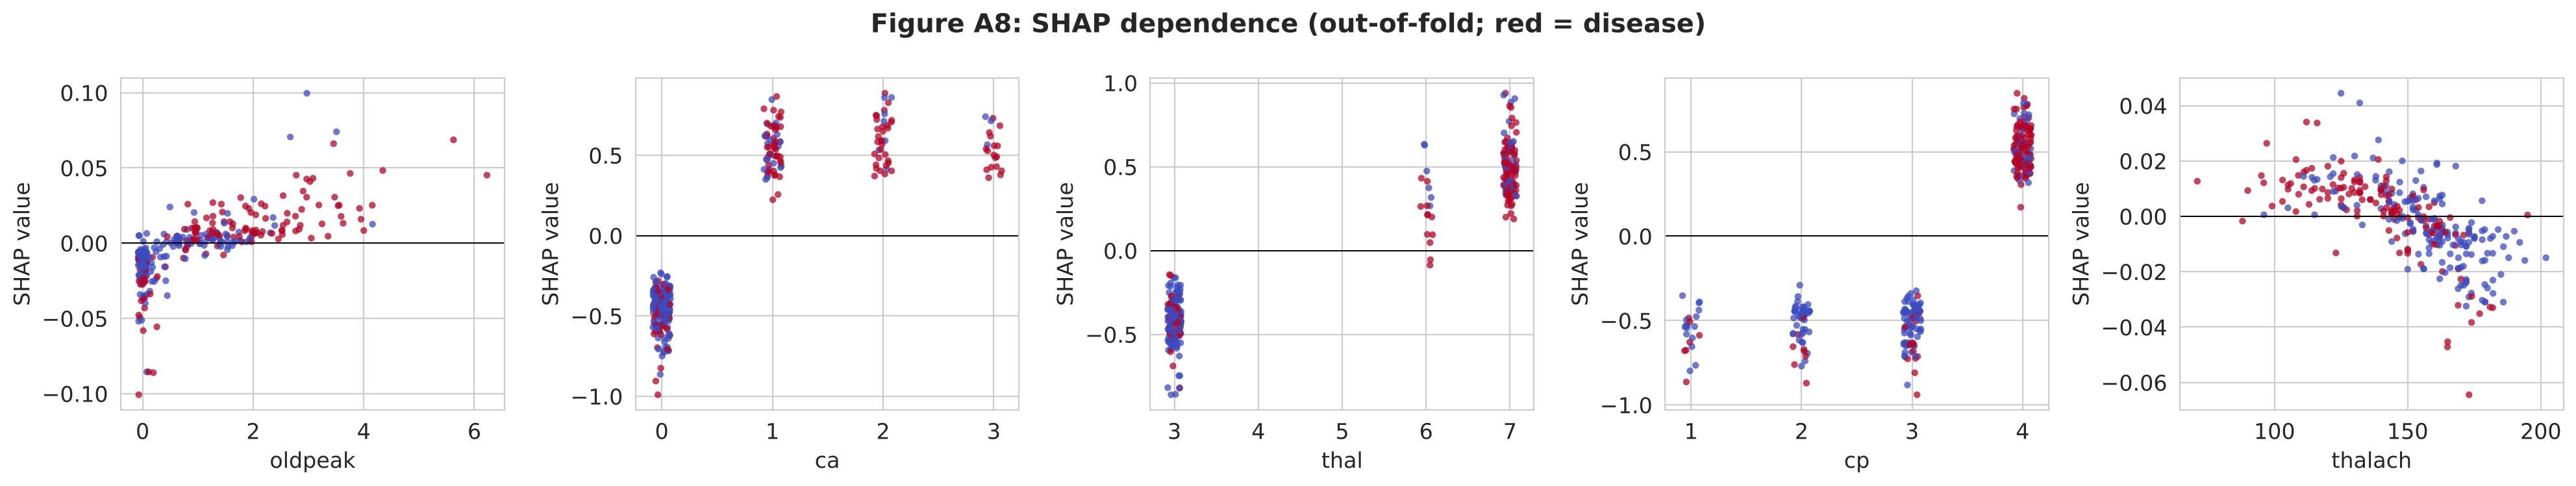
\includegraphics[width=\linewidth]{figA8_shap_dependence.png}
\caption{SHAP dependence for oldpeak, ca, thal, cp and thalach (out-of-fold, repeat 1; red = CAD).}
\label{fig:a8}
\end{figure*}

\begin{figure*}[!t]
\centering
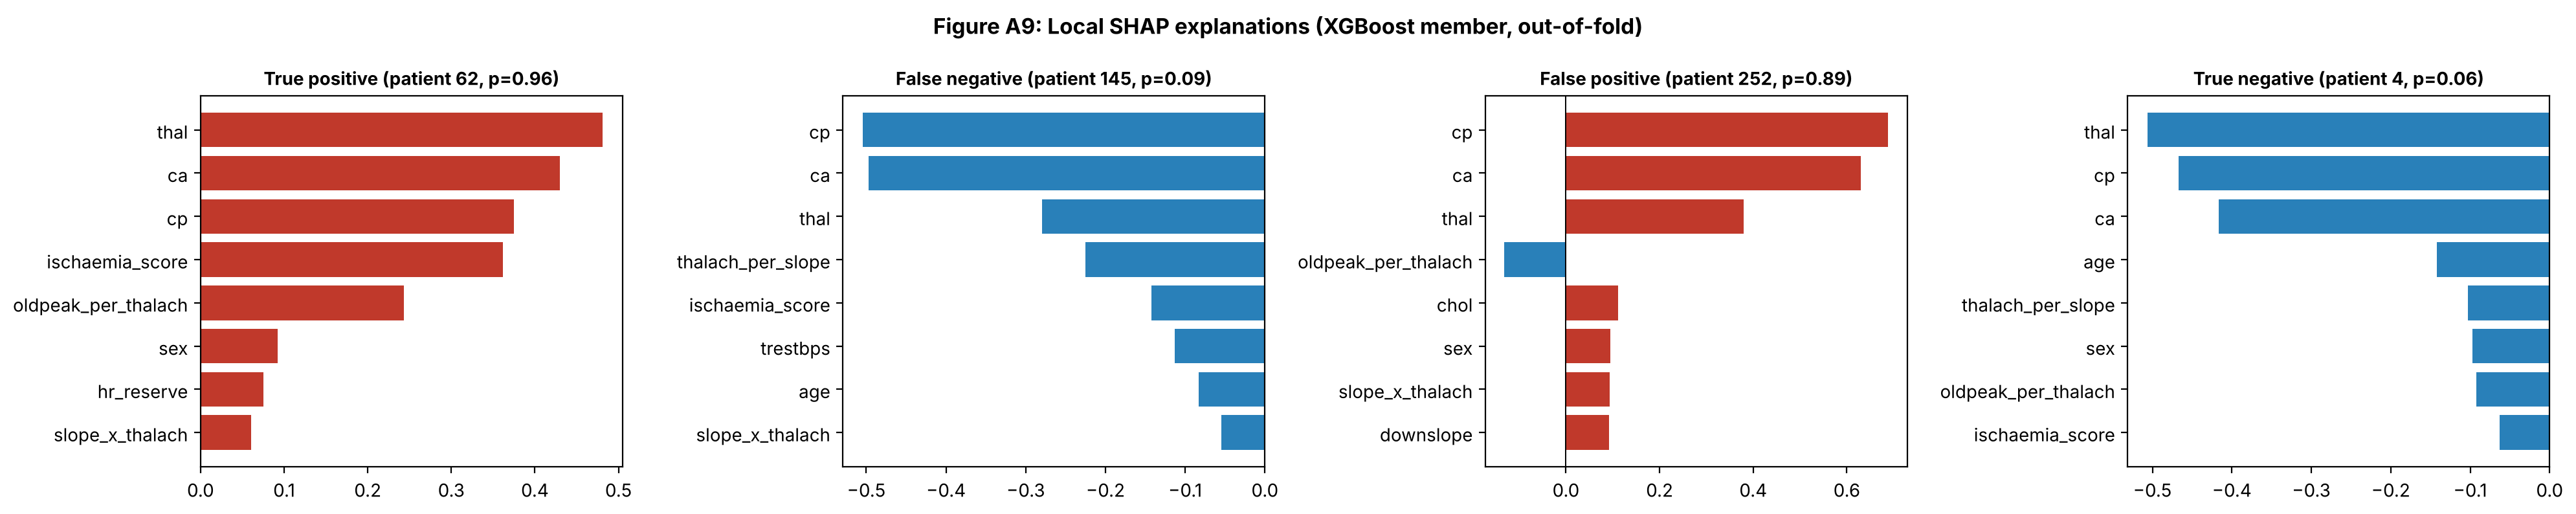
\includegraphics[width=\linewidth]{figA9_shap_local.png}
\caption{Local SHAP explanations (top-8 contributions) for one TP, FN, FP and TN patient.}
\label{fig:a9}
\end{figure*}

\begin{figure}[!t]
\centering
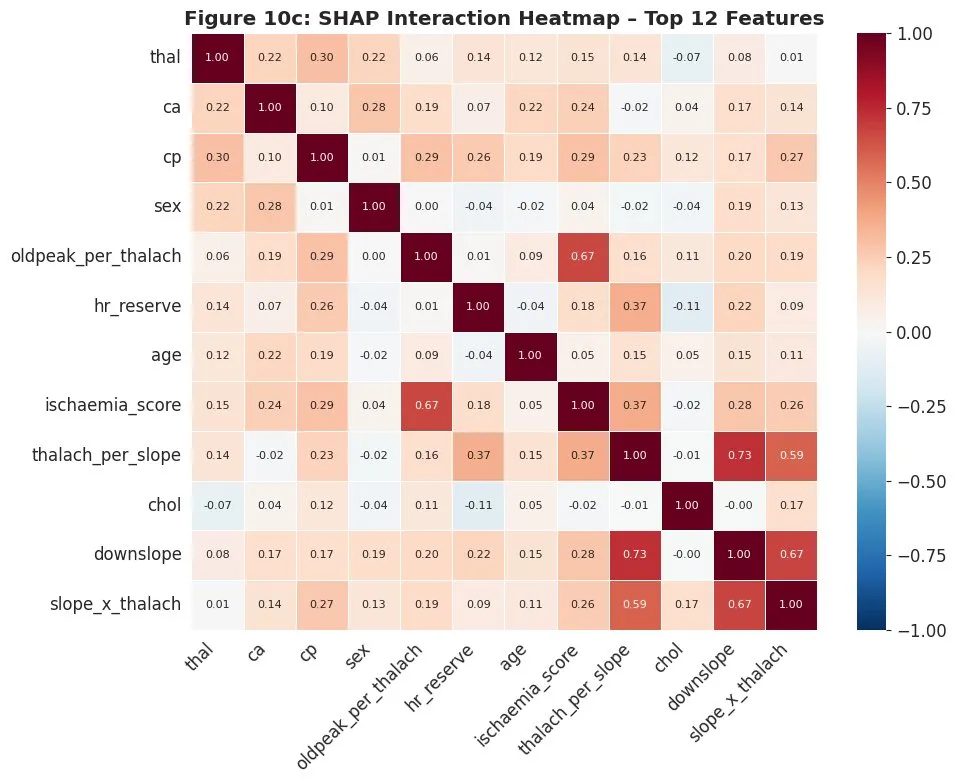
\includegraphics[width=0.9\linewidth]{fig5_shap_heatmap.png}
\caption{Correlation of SHAP values among the top-12 features (v4).}
\label{fig:heatmap}
\end{figure}
